\subsection{Identical labels, different costs}\label{sec:information-loss}
\begin{proposition}\label{prop:label-loss}
Exact one-step Bellman models can have identical strictly improving
targets and identical globally optimal target fits with opposite
teacher-relative cost effects, even with common quadratic curvature,
complete coverage and a teacher in the student class.
\end{proposition}
\begin{proof}
Take three equiprobable contexts, $U=[-1,1]$, teacher zero and constant
students $u=c$. Let
\begin{equation}\label{eq:witness-cost}
 Q_i(u)=(u-\mu_i)^2,\qquad (\mu_1,\mu_2,\mu_3)=(\tau,-1,-1),\quad \tau\geq1.
\end{equation}
For $\rho=0$, the targets are $(1,-1,-1)$ and each improves its teacher.
Their unique minimum-MSE fit is $c=-1/3$, with MSE $8/9<1$. However,
\begin{equation}\label{eq:witness-gap}
 J(-1/3)-J(0)=\frac{2\tau-3}{9},
\end{equation}
which is negative at $\tau=1$ and positive for $\tau>3/2$.

An exact Bellman realization uses $x=(s,y)$, $F(s,y,u)=(s,u)$,
$c_t=u^2$, and $g(s,y)=\mu(s)^2-2\mu(s)y$, with
$\mu(s)=-1+(\tau+1)(s-2)(s-3)/2$. Start uniformly at $(s,0)$,
$s\in\{1,2,3\}$. Total cost is Eq.~\eqref{eq:witness-cost}; the
projected terminal covector is $-2\mu_i$. Sensitivity error and
continuation remainder both vanish.
\end{proof}

At $\tau=10$, the discarded normal term is $18(1-u)$ in the first
context and zero elsewhere. Teacher cost is 34, best target-fit cost
is $323/9=35.888889$, and direct cost minimization in the same constant
class selects $c=1$ with cost $89/3=29.666667$.
For any fixed finite $\rho\geq0$, replacing $\mu_i$ by
$\beta(\tau,-1,-1)_i$, $\beta=1+\rho/2$, keeps the proximal targets
unchanged and gives fitted cost difference $[1+2\beta(\tau-2)]/9>0$
at $\tau=10$. This is an existence construction for each fixed $\rho$.

Retaining $a_z=r_z+\rho_z/2$ and $n_z=\nabla Q_{\rho,z}(u_+)$ restores
\begin{equation}\label{eq:cost-preserving-loss}
 L_{\rm cost}(u;z)=a_z\|u-u_+\|^2+n_z^\top(u-u_+)
                 =Q_{\rho,z}(u)-Q_{\rho,z}(u_+).
\end{equation}
For a fixed state distribution and a class containing the teacher, a
global minimizer cannot increase mean proximal model value. The
teacher's zero proximal penalty gives the same conclusion for the
unregularized model. This is a policy-cost comparison in the exact
one-step example; nonlinear continuation and changed occupancy require
the bounds in \ref{app:transfer}.

On $U=\{u:\|u\|\leq R\}$, write $n_z=-\lambda_z u_+$,
$\lambda_z\geq0$, with $\lambda_z=0$ for interior targets. Expansion gives
\begin{equation}\label{eq:radial-information}
 L_{\rm cost}(u;z)=(a_z+\lambda_z/2)\|u-u_+\|^2
                  +\frac{\lambda_z}{2}(R^2-\|u\|^2).
\end{equation}
Weighted action fitting omits the second term. It can therefore miss
the cost of a student's interior compromise even with the correct weight.

\begin{figure}[htbp]\centering
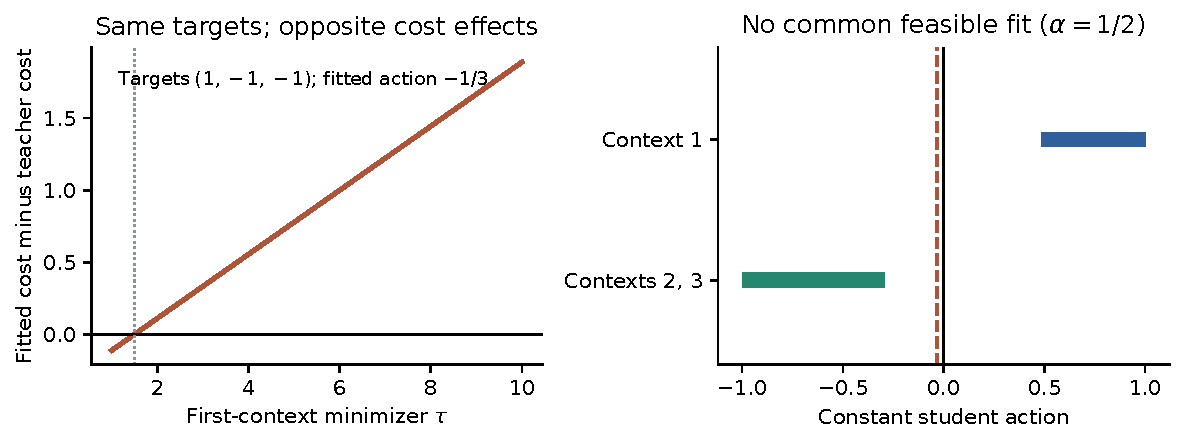
\includegraphics[width=\linewidth]{figures/teaching_information_loss_corrected.pdf}
\caption{Exact constructed failures of the teaching interface. Left:
the same constrained action targets and the same best constant fit have
opposite cost effects as the unconstrained minimizer $\tau$ changes,
with quadratic curvature fixed. Right: each
improvement set is nonempty, but their intersection is empty; the dashed
line is the best constant set-distance fit (\ref{sec:joint-sets}). }
\label{fig:information-loss}
\end{figure}
